%%%%%%%%%%%%%%%%%%%%%%%%%%%%%%%%%%%%%%%%%%%%%%%%%%%%%%%%%%%%%%%%%%%%%%%%%%%%%%%%
% Thesis / Project Report
% LaTeX Template
% Version 2.0 (08/04/16)
%
% Author:
% Siddhant Shrivastava
% https://github.com/sidcode/bits-pilani-thesis-template-latex
%
% This template is heavily based on the work of Darshit Shah, Steven Gunn and Sunil Patel
% Darshit Shah
% https://github.com/darnir/BPHC-LaTeX-Report-Class
% Steven Gunn
% http://users.ecs.soton.ac.uk/srg/softwaretools/document/templates/
% and
% Sunil Patel
% http://www.sunilpatel.co.uk/thesis-template/
%
% License:
% CC BY-NC-SA 4.0 (http://creativecommons.org/licenses/by-nc-sa/4.0/)
%
% Note:
% Make sure to edit document variables in the Thesis.cls file
%
%%%%%%%%%%%%%%%%%%%%%%%%%%%%%%%%%%%%%%%%%%%%%%%%%%%%%%%%%%%%%%%%%%%%%%%%%%%%%%%%

%-------------------------------------------------------------------------------
%	PACKAGES AND OTHER DOCUMENT CONFIGURATIONS
%-------------------------------------------------------------------------------

\documentclass[11pt, a4paper, oneside]{Thesis} % Paper size, default font size
                                               % and one-sided paper

\graphicspath{{Pictures/}} % Specifies the directory where pictures are stored

\usepackage[backend=bibtex]{biblatex}
\bibliography{Bibliography.bib}

\usepackage{hyperref}
\usepackage{enumitem}
\usepackage{mathtools}
\usepackage{etoolbox}% http://ctan.org/pkg/etoolbox
\usepackage{multido}% http://ctan.org/pkg/multido
\usepackage{amsmath} 
\usepackage{graphicx}
\usepackage{lscape}
\usepackage{changepage} 
\usepackage{nccmath} 
\usepackage[table]{xcolor}
\usepackage{times}
\usepackage{helvet}
\usepackage{enumitem}
\usepackage{courier}
\usepackage{caption}
\usepackage{adjustbox}
\usepackage{multicol}
\usepackage{multirow}
\usepackage{afterpage}
\usepackage[table,xcdraw]{xcolor}
\usepackage{float}
\usepackage[caption = false]{subfig}
\usepackage{pdfpages}


\newcommand\Source[1]{\par\scriptsize{\textbf{Source:} \url{#1}\par}}
\newcommand\source[1]{\par\footnotesize{\textbf{Source:} \text{#1}\par}}

\title{\ttitle} % Defines the thesis title - don't touch this

\begin{document}

\frontmatter % Use roman numbering style (i, ii...) for the pre-content pages

\setstretch{1.3} % Line spacing of 1.3

% Define page headers using FancyHdr package and set up for one-sided printing
\fancyhead{} % Clears all page headers and footers
\rhead{\thepage} % Sets the right side header to show the page number
\lhead{} % Clears the left side page header

\pagestyle{fancy} % Finally, use the "fancy" page style to implement the
                  %FancyHdr headers

% Input all the variables used in the document. Please fill out the
% variables.tex file with all your details.
%-------------------------------------------------------------------------------
%	DOCUMENT VARIABLES
%
%	Fill in the lines below to set the various variables for the document
%-------------------------------------------------------------------------------

%-------------------------------------------------------------------------------
% Your thesis title - this is used in the title and abstract
% Command: \ttitle
\thesistitle{Option Pricing using Deep Learning}
%-------------------------------------------------------------------------------
% The document type: Thesis / report, etc.
% Command: \doctype
\documenttype{Undergraduate Thesis}
%-------------------------------------------------------------------------------
% Your supervisor's name - this is used in the title page
% Command: \supname
\supervisor{Prof. N V M \textsc{RAO}}
%-------------------------------------------------------------------------------
% The supervisor's position - Used on Certificate
% Command: \suppos
\supervisorposition{ Professor \\Economics and Finance}
%-------------------------------------------------------------------------------
% Supervisor's institute
% Command: \supinst
\supervisorinstitute{BITS Pilani, Pilani Campus}
%-------------------------------------------------------------------------------
% Your Co-Supervisor's name
% Command: \cosupname
\cosupervisor{Dr. Kokil \textsc{Jaidka}}
%-------------------------------------------------------------------------------
% Co-Supervisor's Position - Used on Certificate
% Command: \cosuppos
\cosupervisorposition{Assistant Professor\\Communications and New Media}
%-------------------------------------------------------------------------------
% Co-Supervisor's Institute
% Command: \cosupinst
\cosupervisorinstitute{National University of Singapore}
%-------------------------------------------------------------------------------
% Your Examiner's name. Not currently used anywhere.
% Command: \examname
\examiner{}
%-------------------------------------------------------------------------------
% Name of your degree
% Command: \degreename
\degree{Bachelor of Engineering (Hons.)}
%-------------------------------------------------------------------------------
% The BITS Course Code for which this report is written
% COmmand: \ccode
\coursecode{BITS F422T}
%-------------------------------------------------------------------------------
% The name of the Course
% Command: \cname
\coursename{Thesis}
%-------------------------------------------------------------------------------
% Your name. Extend manually in case of multiple authors
% Command: \authornames
\authors{Harsh \textsc{Shah}}
%-------------------------------------------------------------------------------
% Your ID Number - used on the Title page and abstract
% Command: \idnum
\IDNumber{2017B3A30650P}
%-------------------------------------------------------------------------------
% Your address
% Command: \addressnames
\addresses{}
%-------------------------------------------------------------------------------
% Your subject area
% Command: \subjectname
\subject{}
%-------------------------------------------------------------------------------
% Keywords for this report.
% Command: \keywordnames
\keywords{}
%-------------------------------------------------------------------------------
% University details
% Command: \univname
\university{\texorpdfstring{\href{http://www.bits-pilani.ac.in/} % URL
                {Birla Institute of Technology and Science Pilani, Pilani Campus}} % University name
                {Birla Institute of Technology and Science Pilani, Pilani Campus}}
%-------------------------------------------------------------------------------
% University details, in Capitals
% Command: \UNIVNAME
\UNIVERSITY{\texorpdfstring{\href{http://www.bits-pilani.ac.in/} % URL
                {BIRLA INSTITUTE OF TECHNOLOGY AND SCIENCE PILANI, PILANI CAMPUS}} % name in capitals
                {BIRLA INSTITUTE OF TECHNOLOGY AND SCIENCE PILANI, PILANI CAMPUS}}
%-------------------------------------------------------------------------------
% Department Details
% Command: \deptname
\department{\texorpdfstring{\href{http://www.bits-pilani.ac.in/pilani/computerscience/ComputerScience} % Your department's URL
                {Department of Economics and Finance}} % Your department's name
                {Department of Economics and Finance}}
%-------------------------------------------------------------------------------
% Department details, in Capitals
% Command: \DEPTNAME
\DEPARTMENT{\texorpdfstring{\href{http://www.bits-pilani.ac.in/pilani/computerscience/ComputerScience} % Your department's URL
                {Department of Economics and Finance}} % Your department's name in capitals
                {Department of Economics and Finance}}
%-------------------------------------------------------------------------------
% Research Group Details
% Command: \groupname
\group{\texorpdfstring{\href{Research Group Web Site URL Here (include http://)}
                {Research Group Name}} % Your research group's name
                {Research Group Name}}
%-------------------------------------------------------------------------------
% Research Group Details, in Capitals
% Command: \GROUPNAME
\GROUP{\texorpdfstring{\href{Research Group Web Site URL Here (include http://)}
                {RESEARCH GROUP NAME (IN BLOCK CAPITALS)}}
                {RESEARCH GROUP NAME (IN BLOCK CAPITALS)}}
%-------------------------------------------------------------------------------
% Faculty details
% Command: \facname
\faculty{\texorpdfstring{\href{Faculty Web Site URL Here (include http://)}
                {Faculty Name}}
                {Faculty Name}}
%-------------------------------------------------------------------------------
% Faculty details, in Capitals
% Command: \FACNAME
\FACULTY{\texorpdfstring{\href{Faculty Web Site URL Here (include http://)}
                {FACULTY NAME (IN BLOCK CAPITALS)}}
                {FACULTY NAME (IN BLOCK CAPITALS)}}
%-------------------------------------------------------------------------------


%-------------------------------------------------------------------------------
%   NON-CONTENT PAGES
%-------------------------------------------------------------------------------
\maketitle
\Declaration
\Certificate
\Quotation{Yesterday is history, Tomorrow is a mystery, and today is a gift. That's why they call it Present.}{Master Oogway}

\begin{abstract}
% The Thesis Abstract is written here (and usually kept to just this page).
% The page is kept centered vertically so can expand into the blank space above
% the title too\ldots
Email is a critical means for asynchronous communication, especially in the workplace. The way people within an organization communicate with each other depends on many factors, including but not limited to email content, historical context, and workplace relations. Prior work in characterizing email communication has focused mainly on linguistic cues but has ignored the signals of pairwise temporal context and workplace relationships that could offer dynamic signals about future behavior, such as replying to emails. This work examines a new dataset of 0.6 million corporate emails exchanged by employees in 2012-2015 to illustrate the importance of influence and interpersonal relationships in a graph-aware temporal framework for predicting enterprise email replies. Incorporating features encoding the sender's influence and likeability in the organizational network in a multimodal framework improves the performance accuracy compared to linguistic features alone. Apart from individual features, we also leverage information related to the relation between sender-receiver pairs, improving the accuracy of predicting subsequent email replies
\end{abstract}

\begin{acknowledgements}

I want to thank Dr. Kokil Jaidka for giving me the opportunity to work under her guidance. She guided me through the research work, helping me understand new concepts and improve my skills. Also, I would like to thank Prof. Surekha Bhanot, who encouraged me to pursue new ideas and provided valuable feedback.

I would like to express gratitude to the National University of Singapore for providing the resources to conduct the research. Additionally, I would like to thank the Electrical and Electronics Department, BITS Pilani for allowing me to pursue the thesis on a topic of my interest. Lastly, I want to express gratitude towards my parents, family and friends who have always been there to support me.
\end{acknowledgements}

%-------------------------------------------------------------------------------
%	LIST OF CONTENTS/FIGURES/TABLES PAGES
%-------------------------------------------------------------------------------

% The page style headers have been "empty" all this time, now use the "fancy"
% headers as defined before to bring them back
\pagestyle{fancy}

\lhead{\emph{Contents}} % Set the left side page header to "Contents"
\tableofcontents % Write out the Table of Contents

% Set the left side page header to "List of Figures"
\lhead{\emph{List of Figures}}
\listoffigures % Write out the List of Figures

 % Set the left side page header to "List of Tables"
\lhead{\emph{List of Tables}}
\listoftables % Write out the List of Tables

%-------------------------------------------------------------------------------
%	ABBREVIATIONS
%-------------------------------------------------------------------------------

\clearpage % Start a new page

 % Set the line spacing to 1.5, this makes the following tables easier to read
\setstretch{1.5}

\lhead{\emph{Abbreviations}} % Set the left side page header to "Abbreviations"
\listofsymbols{ll} % Include a list of Abbreviations (a table of two columns)
{
\textbf{SVC} & \textbf{S}upport \textbf{V}ector \textbf{C}lassifier \\
\textbf{DNN} & \textbf{D}eep \textbf{N}eural \textbf{N}etwork \\
\textbf{TF-IDF} & \textbf{T}erm \textbf{F}requency -  \textbf{I}nverse \textbf{D}ocument \textbf{F}requency \\
\textbf{NLP} & \textbf{N}atural \textbf{L}anguage \textbf{P}rocessing \\
\textbf{CNN} & \textbf{C}onvolutional \textbf{N}eural \textbf{N}etwork \\
\textbf{RNN} & \textbf{R}ecurrent \textbf{N}eural \textbf{N}etwork \\
\textbf{LSTM} & \textbf{L}ong \textbf{S}hort \textbf{T}erm \textbf{M}emory\\
\textbf{GNN} & \textbf{G}raph \textbf{N}eural \textbf{N}etwork \\
\textbf{GCN} & \textbf{G}raph \textbf{C}onvolutional \textbf{N}etwork \\
\textbf{BERT} & \textbf{B}idirectional \textbf{E}ncoder \textbf{R}epresentations from \textbf{T}ransformers\\
\textbf{RoBERTa} & \textbf{R}obustly \textbf{O}ptimised \textbf{BERT} Pretraining \textbf{A}pproach\\
\textbf{CSV} & \textbf{C}omma \textbf{S}eperated \textbf{V}alues \\
\textbf{LIWC} &   \textbf{L}inguistic \textbf{I}nquiry and \textbf{W}ord \textbf{C}ount \\
\textbf{SNA} & \textbf{S}ocial \textbf{N}etwork \textbf{A}nalysis

%\textbf{Acronym} & \textbf{W}hat (it) \textbf{S}tands \textbf{F}or \\
}

%-------------------------------------------------------------------------------
%	PHYSICAL CONSTANTS/OTHER DEFINITIONS
%-------------------------------------------------------------------------------

% \clearpage % Start a new page

% % Set the left side page header to "Physical Constants"
% \lhead{\emph{Notation}}

%  % Include a list of Physical Constants (a four column table)
% \listofconstants{lrcl}
% {
% Speed of Light & $c$ & $=$ & $2.997\ 924\ 58\times10^{8}\ \mbox{ms}^{-\mbox{s}}$ (exact)\\
% % Constant Name & Symbol & = & Constant Value (with units) \\
% }

%-------------------------------------------------------------------------------
%	SYMBOLS
%-------------------------------------------------------------------------------

% \clearpage % Start a new page

% \lhead{\emph{Glossary}} % Set the left side page header to "Symbols"

% \listofnomenclature % List the nomenclature. (We use the glossaries package)

%-------------------------------------------------------------------------------
%	DEDICATION
%-------------------------------------------------------------------------------

\setstretch{1.5} % Return the line spacing back to 1.3

\pagestyle{empty} % Page style needs to be empty for this page

% Dedication text
\Dedicatory{Dedicated to my Parents}

\addtocontents{toc}{\vspace{2em}} % Add a gap in the Contents, for aesthetics

%-------------------------------------------------------------------------------
%	THESIS CONTENT - CHAPTERS
%-------------------------------------------------------------------------------

\mainmatter % Begin numeric (1,2,3...) page numbering

\pagestyle{fancy} % Return the page headers back to the "fancy" style

% Include the chapters of the thesis as separate files from the Chapters folder
% Uncomment the lines as you write the chapters

% Chapter 1

\chapter{Introduction} % Main chapter title

\label{Chapter1} % For referencing the chapter elsewhere, use \ref{Chapter1} 

\lhead{Chapter 1. \emph{Introduction}} % This is for the header on each page - perhaps a shortened title

%----------------------------------------------------------------------------------------

\section{Email Reply Prediction}

Email is a critical means for asynchronous communication, especially in the workplace. In recent times, many corporations have started shifting to remote or hybrid work which involves a lot of communication between the employees over different channels out of which email is often the primary one. Accurately predicting whether a sent mail will receive a reply or not can help the involved parties manage their time and work efficiently.   

The way people within an organization communicate with each other depends on many factors, including but not limited to email content, historical context, and workplace relations. Prior work in characterizing email communication has focused mainly on linguistic cues but has ignored the signals of pairwise temporal context and workplace relationships that could offer dynamic signals about future behavior, such as replying to emails. This work examines a new dataset of 0.6 million corporate emails exchanged by employees in 2012-2015 to illustrate the importance of influence and interpersonal relationships in a graph-aware temporal framework for predicting enterprise email replies. 

Incorporating features encoding the sender's influence and likeability in the organizational network in a multimodal framework improves the performance accuracy compared to linguistic features alone. Apart from individual features, we also leverage information related to the relation between sender-receiver pairs, improving the accuracy of predicting subsequent email replies.

% Welcome to this \LaTeX{} Thesis Template, a beautiful and easy to use template for writing a thesis using the \LaTeX{} typesetting system.

% If you are writing a thesis (or will be in the future) and its subject is technical or mathematical (though it doesn't have to be), then creating it in \LaTeX{} is highly recommended as a way to make sure you can just get down to the essential writing without having to worry over formatting or wasting time arguing with your word processor.

% \LaTeX{} is easily able to professionally typeset documents that run to hundreds or thousands of pages long. With simple mark-up commands, it automatically sets out the table of contents, margins, page headers and footers and keeps the formatting consistent and beautiful. One of its main strengths is the way it can easily typeset mathematics, even \emph{heavy} mathematics. Even if those equations are the most horribly twisted and most difficult mathematical problems that can only be solved on a super-computer, you can at least count on \LaTeX{} to make them look stunning.

%----------------------------------------------------------------------------------------

\section{Commercial \& Research Applications}

Commercial products like Google Mail and Outlook are widely used by corporations for a majority of their work related communication. Incorporating the model proposed into these existing email services directly or via a browser add-on is not a very complex task. Based on who the sender and receiver are, the model can predict whether the current email body will result in a reply or not. This also allows the user to tweak the text until a satisfactory number is predicted as the probability of getting a reply.  

While this work poses the problem as a binary classification task where a 0 and 1 mean not getting and getting a reply respectively, the model can also be modified to perform a regression task to predict the time it will take for the receiver to reply to that mail. Furthermore, if the replies of the receiver are present, one can also train a generative language model to generate contextual replies to a given mail.

\section{Literature Review}

A lot of prior work exists on the topic of email classification. Sarrafzadeh et al. \cite{10.1145/3289600.3291028} performed qualitative and quantitative study to find out how often emails are deferred or ignored. The Enron corpus\cite{DBLP:conf/ecml/KlimtY04} released in 2004 also dives into classifying emails. Apart from classification, there is also email intent extraction and analysis. Sappelli et al. \cite{maya_email_intent} demonstrated that tasks and intents in emails can be extracted with high accuracy. Other work tries to rank all unread emails by ranking them according to their importance\cite{36955}.  

Looking at the specific topic of email reply probability prediction, Liu et al. \cite{10.1145/3077136.3080782} proposed a model to predict the likeliness and time that a recipient may take to reply to a certain mail. This work provided insights about importance of different features like number of attachments and email body length.
Mukherjee et al. \cite{mukherjee2019contentbased} decided to approach this problem as content-based recommendation. To achieve this, they compute user representation by looking at their inbox. Using this, they compute similarity between the email and the user's inbox, which helps improve the prediction accuracy. 

Taking inspiration from prior research done on this topic, the proposed model incorporates not just the mail text and the user inbox when predicting the probabilty, but also looks at social graph, temporal and workplace relation related features.

\section{Thesis Outline}

The next few chapters cover the theory and concepts used in this work.

\hyperref[Chapter2]{Chapter 2} contains the basics of various Deep Learning-based architectures used in Natural Language Processing, starting from Vanilla Neural Networks and building up to the current State-of-the-Art Transformer models like BERT. %cite BERT  

\hyperref[Chapter3]{Chapter 3} explores the dataset used in this work. A lot of numerical and categorical features apart from the text used in the model(s) have been derived from this data which are also discussed in this chapter.

\hyperref[Chapter4]{Chapter 4} contains the details of the baseline and multimodal models which have been used to run the experiments

\hyperref[Chapter5]{Chapter 5} has the results and discussion. 

\hyperref[Chapter6]{Chapter 6}  concludes the work presented in the previous chapters and provides a direction for further research in this topic - particularly with Graph Neural Networks.


% _______________________________
% % \LaTeX{} is not a WYSIWYG (What You See is What You Get) program, unlike word processors such as Microsoft Word or Apple's Pages. Instead, a document written for \LaTeX{} is actually a simple, plain text file that contains \emph{no formatting}. You tell \LaTeX{} how you want the formatting in the finished document by writing in simple commands amongst the text, for example, if I want to use \textit{italic text for emphasis}, I write the `$\backslash$\texttt{textit}\{\}' command and put the text I want in italics in between the curly braces. This means that \LaTeX{} is a ``mark-up'' language, very much like HTML.

% \subsection{A (not so short) Introduction to \LaTeX{}}

% If you are new to \LaTeX{}, there is a very good eBook -- freely available online as a PDF file -- called, ``The Not So Short Introduction to \LaTeX{}''. The book's title is typically shortened to just ``lshort''. You can download the latest version (as it is occasionally updated) from here:\\
% \href{http://www.ctan.org/tex-archive/info/lshort/english/lshort.pdf}{\texttt{http://www.ctan.org/tex-archive/info/lshort/english/lshort.pdf}}

% It is also available in several other languages. Find yours from the list on this page:\\
% \href{http://www.ctan.org/tex-archive/info/lshort/}{\texttt{http://www.ctan.org/tex-archive/info/lshort/}}

% It is recommended to take a little time out to learn how to use \LaTeX{} by creating several, small `test' documents. Making the effort now means you're not stuck learning the system when what you \emph{really} need to be doing is writing your thesis.

% \subsection{A Short Math Guide for \LaTeX{}}

% If you are writing a technical or mathematical thesis, then you may want to read the document by the AMS (American Mathematical Society) called, ``A Short Math Guide for \LaTeX{}''. It can be found online here:\\
% \href{http://www.ams.org/tex/amslatex.html}{\texttt{http://www.ams.org/tex/amslatex.html}}\\
% under the ``Additional Documentation'' section towards the bottom of the page.

% \subsection{Common \LaTeX{} Math Symbols}
% There are a multitude of mathematical symbols available for \LaTeX{} and it would take a great effort to learn the commands for them all. The most common ones you are likely to use are shown on this page:\\
% \href{http://www.sunilpatel.co.uk/latexsymbols.html}{\texttt{http://www.sunilpatel.co.uk/latexsymbols.html}}

% You can use this page as a reference or crib sheet, the symbols are rendered as large, high quality images so you can quickly find the \LaTeX{} command for the symbol you need.

% \subsection{\LaTeX{} on a Mac}
 
% The \LaTeX{} package is available for many systems including Windows, Linux and Mac OS X. The package for OS X is called MacTeX and it contains all the applications you need -- bundled together and pre-customised -- for a fully working \LaTeX{} environment and workflow.
 
% MacTeX includes a dedicated \LaTeX{} IDE (Integrated Development Environment) called ``TeXShop'' for writing your `\texttt{.tex}' files and ``BibDesk'': a program to manage your references and create your bibliography section just as easily as managing songs and creating playlists in iTunes.

% %----------------------------------------------------------------------------------------

% \section{Getting Started with this Template}

% If you are familiar with \LaTeX{}, then you can familiarise yourself with the contents of the Zip file and the directory structure and then place your own information into the `\texttt{Thesis.cls}' file. Section \ref{FillingFile} on page \pageref{FillingFile} tells you how to do this. Make sure you read section \ref{ThesisConventions} about thesis conventions to get the most out of this template and then get started with the `\texttt{Thesis.tex}' file straightaway.

% If you are new to \LaTeX{} it is recommended that you carry on reading through the rest of the information in this document.

% \subsection{About this Template}

% This \LaTeX{} Thesis Template is originally based and created around a \LaTeX{} style file created by Steve R.\ Gunn from the University of Southampton (UK), department of Electronics and Computer Science. You can find his original thesis style file at his site, here:\\
% \href{http://www.ecs.soton.ac.uk/~srg/softwaretools/document/templates/}{\texttt{http://www.ecs.soton.ac.uk/$\sim$srg/softwaretools/document/templates/}}

% My thesis originally used the `\texttt{ecsthesis.cls}' from his list of styles. However, I knew \LaTeX{} could still format better. To get the look I wanted, I modified his style and also created a skeleton framework and folder structure to place the thesis files in.

% This Thesis Template consists of that modified style, the framework and the folder structure. All the work that has gone into the preparation and groundwork means that all you have to bother about is the writing.

% Before you begin using this template you should ensure that its style complies with the thesis style guidelines imposed by your institution. In most cases this template style and layout will be suitable. If it is not, it may only require a small change to bring the template in line with your institution's recommendations.

% %----------------------------------------------------------------------------------------

% \section{What this Template Includes}

% \subsection{Folders}

% This template comes as a single Zip file that expands out to many files and folders. The folder names are mostly self-explanatory:

% \textbf{Appendices} -- this is the folder where you put the appendices. Each appendix should go into its own separate `\texttt{.tex}' file. A template is included in the directory.

% \textbf{Chapters} -- this is the folder where you put the thesis chapters. A thesis usually has about seven chapters, though there is no hard rule on this. Each chapter should go in its own separate `\texttt{.tex}' file and they usually are split as:
% \begin{itemize}
% \item Chapter 1: Introduction to the thesis topic
% \item Chapter 2: Background information and theory
% \item Chapter 3: (Laboratory) experimental setup
% \item Chapter 4: Details of experiment 1
% \item Chapter 5: Details of experiment 2
% \item Chapter 6: Discussion of the experimental results
% \item Chapter 7: Conclusion and future directions
% \end{itemize}
% This chapter layout is specialised for the experimental sciences.

% \textbf{Figures} -- this folder contains all figures for the thesis. These are the final images that will go into the thesis document.

% \textbf{Primitives} -- this is the folder that contains scraps, particularly because one final image in the `Figures' folder may be made from many separate images and photos, these source images go here. This keeps the intermediate files separate from the final thesis figures.

% \subsection{Files}

% Included are also several files, most of them are plain text and you can see their contents in a text editor. Luckily, many of them are auxiliary files created by \LaTeX{} or BibTeX and which you don't need to bother about:

% \textbf{Bibliography.bib} -- this is an important file that contains all the bibliographic information and references that you will be citing in the thesis for use with BibTeX. You can write it manually, but there are reference manager programs available that will create and manage it for you. Bibliographies in \LaTeX{} are a large subject and you may need to read about BibTeX before starting with this.

% \textbf{Thesis.cls} -- this is an important file. It is the style file that tells \LaTeX{} how to format the thesis. You will also need to open this file in a text editor and fill in your own information (such as name, department, institution). Luckily, this is not too difficult and is explained in section \ref{FillingFile} on page \pageref{FillingFile}.

% \textbf{Thesis.pdf} -- this is your beautifully typeset thesis (in the PDF file format) created by \LaTeX{}.

% \textbf{Thesis.tex} -- this is an important file. This is the file that you tell \LaTeX{} to compile to produce your thesis as a PDF file. It contains the framework and constructs that tell \LaTeX{} how to layout the thesis. It is heavily commented so you can read exactly what each line of code does and why it is there. After you put your own information into the `\texttt{Thesis.cls}' file, go to this file and begin filling it in -- you have now started your thesis!

% \textbf{vector.sty} -- this is a \LaTeX{} package, it tells \LaTeX{} how to typeset mathematical vectors. Using this package is very easy and you can read the documentation on the site (you just need to look at the `\texttt{vector.pdf}' file):\\
% \href{http://www.ctan.org/tex-archive/macros/latex/contrib/vector/}{\texttt{http://www.ctan.org/tex-archive/macros/latex/contrib/vector/}}

% \textbf{lstpatch.sty} -- this is a \LaTeX{} package required by this LaTeX template and is included as not all \TeX{} distributions have it installed by default. You do not need to modify this file.

% Files that are \emph{not} included, but are created by \LaTeX{} as auxiliary files include:

% \textbf{Thesis.aux} -- this is an auxiliary file generated by \LaTeX{}, if it is deleted \LaTeX{} simply regenerates it when you run the main `\texttt{.tex}' file.

% \textbf{Thesis.bbl} -- this is an auxiliary file generated by BibTeX, if it is deleted, BibTeX simply regenerates it when you run the main tex file. Whereas the `\texttt{.bib}' file contains all the references you have, this `\texttt{.bbl}' file contains the references you have actually cited in the thesis and is used to build the bibliography section of the thesis.

% \textbf{Thesis.blg} -- this is an auxiliary file generated by BibTeX, if it is deleted BibTeX simply regenerates it when you run the main `\texttt{.tex}' file.

% \textbf{Thesis.lof} -- this is an auxiliary file generated by \LaTeX{}, if it is deleted \LaTeX{} simply regenerates it when you run the main `\texttt{.tex}' file. It tells \LaTeX{} how to build the `List of Figures' section.

% \textbf{Thesis.log} -- this is an auxiliary file generated by \LaTeX{}, if it is deleted \LaTeX{} simply regenerates it when you run the main `\texttt{.tex}' file. It contains messages from \LaTeX{}, if you receive errors and warnings from \LaTeX{}, they will be in this `\texttt{.log}' file.

% \textbf{Thesis.lot} -- this is an auxiliary file generated by \LaTeX{}, if it is deleted \LaTeX{} simply regenerates it when you run the main `\texttt{.tex}' file. It tells \LaTeX{} how to build the `List of Tables' section.

% \textbf{Thesis.out} -- this is an auxiliary file generated by \LaTeX{}, if it is deleted \LaTeX{} simply regenerates it when you run the main `\texttt{.tex}' file.


% So from this long list, only the files with the `\texttt{.sty}', `\texttt{.bib}', `\texttt{.cls}' and `\texttt{.tex}' extensions are the most important ones. The other auxiliary files can be ignored or deleted as \LaTeX{} and BibTeX will regenerate them.

% %----------------------------------------------------------------------------------------

% \section{Filling in the `\texttt{Thesis.cls}' File}\label{FillingFile}

% You will need to personalise the thesis template and make it your own by filling in your own information. This is done by editing the `\texttt{Thesis.cls}' file in a text editor.

% Open the file and scroll down, past all the `$\backslash$\texttt{newcommand}\ldots' items until you see the entries for `\texttt{University Name}', `\texttt{Department Name}', etc\ldots.

% Fill out the information about your group and institution and ensure you keep to block capitals where it asks you to. You can also insert web links, if you do, make sure you use the full URL, including the `\texttt{http://}' for this.

% The last item you should need to fill in is the Faculty Name (in block capitals). When you have done this, save the file and recompile `\texttt{Thesis.tex}'. All the information you filled in should now be in the PDF, complete with web links. You can now begin your thesis proper!

% %----------------------------------------------------------------------------------------

% \section{The `\texttt{Thesis.tex}' File Explained}

% The \texttt{Thesis.tex} file contains the structure of the thesis. There are plenty of written comments that explain what pages, sections and formatting the \LaTeX{} code is creating. Initially there seems to be a lot of \LaTeX{} code, but this is all formatting, and it has all been taken care of so you don't have to do it.

% Begin by checking that your information on the title page is correct. For the thesis declaration, your institution may insist on something different than the text given. If this is the case, just replace what you see with what is required.

% Then comes a page which contains a funny quote. You can put your own, or quote your favourite scientist, author, person, etc\ldots Make sure to put the name of the person who you took the quote from.

% Next comes the acknowledgements. On this page, write about all the people who you wish to thank (not forgetting parents, partners and your advisor/supervisor).

% The contents pages, list of figures and tables are all taken care of for you and do not need to be manually created or edited. The next set of pages are optional and can be deleted since they are for a more technical thesis: insert a list of abbreviations you have used in the thesis, then a list of the physical constants and numbers you refer to and finally, a list of mathematical symbols used in any formulae. Making the effort to fill these tables means the reader has a one-stop place to refer to instead of searching the internet and references to try and find out what you meant by certain abbreviations or symbols.

% The list of symbols is split into the Roman and Greek alphabets. Whereas the abbreviations and symbols ought to be listed in alphabetical order (and this is \emph{not} done automatically for you) the list of physical constants should be grouped into similar themes.

% The next page contains a one line dedication. Who will you dedicate your thesis to?

% Finally, there is the section where the chapters are included. Uncomment the lines (delete the `\texttt{\%}' character) as you write the chapters. Each chapter should be written in its own file and put into the `Chapters' folder and named `\texttt{Chapter1}', `\texttt{Chapter2}, etc\ldots Similarly for the appendices, uncomment the lines as you need them. Each appendix should go into its own file and placed in the `Appendices' folder.

% After the preamble, chapters and appendices finally comes the bibliography. The bibliography style (called `\texttt{unsrtnat}') is used for the bibliography and is a fully featured style that will even include links to where the referenced paper can be found online. Do not under estimate how grateful you reader will be to find that a reference to a paper is just a click away. Of course, this relies on you putting the URL information into the BibTeX file in the first place.

% %----------------------------------------------------------------------------------------

% \section{Thesis Features and Conventions}\label{ThesisConventions}

% To get the best out of this template, there are a few conventions that you may want to follow.

% One of the most important (and most difficult) things to keep track of in such a long document as a thesis is consistency. Using certain conventions and ways of doing things (such as using a Todo list) makes the job easier. Of course, all of these are optional and you can adopt your own method.

% \subsection{Printing Format}

% This thesis template is designed for single sided printing as most theses are printed and bound this way. This means that the left margin is always wider than the right (for binding). Four out of five people will now judge the margins by eye and think, ``I never 
% noticed that before.''.

% The headers for the pages contain the page number on the right side (so it is easy to flick through to the page you want) and the chapter name on the left side.

% The text is set to 11 point and a line spacing of 1.3. Generally, it is much more readable to have a smaller text size and wider gap between the lines than it is to have a larger text size and smaller gap. Again, you can tune the text size and spacing should you want or need to. The text size can be set in the options for the `$\backslash$\texttt{documentclass}' command at the top of the `\texttt{Thesis.tex}' file and the spacing can be changed by setting a different value in the `$\backslash$\texttt{setstretch}' commands (scattered throughout the `\texttt{Thesis.tex}' file).

% \subsection{Using US Letter Paper}

% The paper size used in the template is A4, which is a common -- if not standard -- size in Europe. If you are using this thesis template elsewhere and particularly in the United States, then you may have to change the A4 paper size to the US Letter size. Unfortunately, this is not as simple as replacing instances of `\texttt{a4paper}' with `\texttt{letterpaper}'.

% This is because the final PDF file is created directly from the \LaTeX{} source using a program called `\texttt{pdfTeX}' and in certain conditions, paper size commands are ignored and all documents are created with the paper size set to the size stated in the configuration file for pdfTeX (called `\texttt{pdftex.cfg}').

% What needs to be done is to change the paper size in the configuration file for \texttt{pdfTeX} to reflect the letter size. There is an excellent tutorial on how to do this here: \\
% \href{http://www.physics.wm.edu/~norman/latexhints/pdf_papersize.html}{\texttt{http://www.physics.wm.edu/$\sim$norman/latexhints/pdf\_papersize.html}}

% It may be sufficient just to replace the dimensions of the A4 paper size with the US Letter size in the \texttt{pdftex.cfg} file. Due to the differences in the paper size, the resulting margins may be different to what you like or require (as it is common for Institutions to dictate certain margin sizes). If this is the case, then the margin sizes can be tweaked by opening up the \texttt{Thesis.cls} file and searching for the line beginning with, `$\backslash$\texttt{setmarginsrb}' (not very far down from the top), there you will see the margins specified. Simply change those values to what you need (or what looks good) and save. Now your document should be set up for US Letter paper size with suitable margins.

% \subsection{References}

% The `\texttt{natbib}' package is used to format the bibliography and inserts references such as this one \cite{cmu-malware}. The options used in the `\texttt{Thesis.tex}' file mean that the references are listed in numerical order as they appear in the text. Multiple references are rearranged in numerical order (e.g. \cite{kendall2007practical}). This is done automatically for you. To see how you use references, have a look at the `\texttt{Chapter1.tex}' source file. Many reference managers allow you to simply drag the reference into the document as you type.

% Scientific references should come \emph{before} the punctuation mark if there is one (such as a comma or period). The same goes for footnotes\footnote{Such as this footnote, here down at the bottom of the page.}. You can change this but the most important thing is to keep the convention consistent throughout the thesis. Footnotes themselves should be full, descriptive sentences (beginning with a capital letter and ending with a full stop).

% To see how \LaTeX{} typesets the bibliography, have a look at the very end of this document (or just click on the reference number links).

% \subsection{Figures}

% There will hopefully be many figures in your thesis (that should be placed in the `Figures' folder). The way to insert figures into your thesis is to use a code template like this:
% \begin{verbatim}
% \begin{figure}[htbp]
%   \centering
%     
\includegraphics{Figures/Electron.pdf}
%     \rule{35em}{0.5pt}
%   \caption[An Electron]{An electron (artist's impression).}
%   \label{fig:Electron}
% \end{figure}
% \end{verbatim}
% Also look in the source file. Putting this code into the source file produces the picture of the electron that you can see in the figure below.

% \begin{figure}[htbp]
% 	\centering
% 		
\includegraphics{Figures/Electron.pdf}
% 		\rule{35em}{0.5pt}
% 	\caption[An Electron]{An electron (artist's impression).}
% 	\label{fig:Electron}
% \end{figure}

% Sometimes figures don't always appear where you write them in the source. The placement depends on how much space there is on the page for the figure. Sometimes there is not enough room to fit a figure directly where it should go (in relation to the text) and so \LaTeX{} puts it at the top of the next page. Positioning figures is the job of \LaTeX{} and so you should only worry about making them look good!

% Figures usually should have labels just in case you need to refer to them (such as in Figure \ref{fig:Electron}). The `$\backslash$\texttt{caption}' command contains two parts, the first part, inside the square brackets is the title that will appear in the `List of Figures', and so should be short. The second part in the curly brackets should contain the longer and more descriptive caption text.

% The `$\backslash$\texttt{rule}' command is optional and simply puts an aesthetic horizontal line below the image. If you do this for one image, do it for all of them.

% The \LaTeX{} Thesis Template is able to use figures that are either in the PDF or JPEG file format.

% \subsection{Typesetting mathematics}

% If your thesis is going to contain heavy mathematical content, be sure that \LaTeX{} will make it look beautiful, even though it won't be able to solve the equations for you.

% The ``Not So Short Introduction to \LaTeX{}'' (available \href{http://www.ctan.org/tex-archive/info/lshort/english/lshort.pdf}{here}) should tell you everything you need to know for most cases of typesetting mathematics. If you need more information, a much more thorough mathematical guide is available from the AMS called, ``A Short Math Guide to \LaTeX{}'' and can be downloaded from:\\
% \href{ftp://ftp.ams.org/pub/tex/doc/amsmath/short-math-guide.pdf}{\texttt{ftp://ftp.ams.org/pub/tex/doc/amsmath/short-math-guide.pdf}}

% There are many different \LaTeX{} symbols to remember, luckily you can find the most common symbols \href{http://www.sunilpatel.co.uk/latexsymbols.html}{here}. You can use the web page as a quick reference or crib sheet and because the symbols are grouped and rendered as high quality images (each with a downloadable PDF), finding the symbol you need is quick and easy.

% You can write an equation, which is automatically given an equation number by \LaTeX{} like this:
% \begin{verbatim}
% \begin{equation}
% E = mc^{2}
%   \label{eqn:Einstein}
% \end{equation}
% \end{verbatim}

% This will produce Einstein's famous energy-matter equivalence equation:
% \begin{equation}
% E = mc^{2}
% \label{eqn:Einstein}
% \end{equation}

% All equations you write (which are not in the middle of paragraph text) are automatically given equation numbers by \LaTeX{}. If you don't want a particular equation numbered, just put the command, `$\backslash$\texttt{nonumber}' immediately after the equation.

% %----------------------------------------------------------------------------------------

% \section{Sectioning and Subsectioning}

% You should break your thesis up into nice, bite-sized sections and subsections. \LaTeX{} automatically builds a table of Contents by looking at all the `$\backslash$\texttt{chapter}$\{\}$', `$\backslash$\texttt{section}$\{\}$' and `$\backslash$\texttt{subsection}$\{\}$' commands you write in the source.

% The table of Contents should only list the sections to three (3) levels. A `$\backslash$\texttt{chapter}$\{\}$' is level one (1). A `$\backslash$\texttt{section}$\{\}$' is level two (2) and so a `$\backslash$\texttt{subsection}$\{\}$' is level three (3). In your thesis it is likely that you will even use a `$\backslash$\texttt{subsubsection}$\{\}$', which is level four (4). Adding all these will create an unnecessarily cluttered table of Contents and so you should use the `$\backslash$\texttt{subsubsection$^{*}\{\}$}' command instead (note the asterisk). The asterisk ($^{*}$) tells \LaTeX{} to omit listing the subsubsection in the Contents, keeping it clean and tidy.

% %----------------------------------------------------------------------------------------

% \section{In Closing}

% You have reached the end of this mini-guide. You can now rename or overwrite this pdf file and begin writing your own `\texttt{Chapter1.tex}' and the rest of your thesis. The easy work of setting up the structure and framework has been taken care of for you. It's now your job to fill it out!

% Good luck and have lots of fun!

% \begin{flushright}
% Guide written by ---\\
% Sunil Patel: \href{http://www.sunilpatel.co.uk}{www.sunilpatel.co.uk}
% \end{flushright}

% Chapter 1

\chapter{Background Concepts} % Main chapter title

\label{Chapter2} % For referencing the chapter elsewhere, use \ref{Chapter1} 

\lhead{Chapter 2. \emph{Background Concepts}} % This is for the header on each page - perhaps a shortened title

%----------------------------------------------------------------------------------------
\section{Neural Networks}

Machine learning research has been growing rapidly over the past decade, with most of this progress coming from deep neural networks (DNNs). These models are powerful tools that can learn to recognize patterns in data, and they have been instrumental in many recent successes in the field.

Neural networks have been studied and developed for many years, with early work on the topic appearing in the late 1950s\cite{Rosenblatt1958ThePA}. One of the most influential papers in this field is the 1986 paper\cite{Rumelhart1986LearningRB}, which introduced the backpropagation algorithm for updating the weights of the network using partial derivatives. This paper and its methods are still used today in modern deep learning.

% This method was successful for shallower networks, but it was very difficult to train deeper networks because of the computational limits at that time. DNNs did not gain much popularity until the early 2010s when the growth of data and increased computational power resulted in a boom in this field.

\subsection{Neurons}

Neural networks were designed to simulate the way the brain learns. This is why they are structured like interconnected neurons passing information, similar to how neurons fire in the human brain. 
A neuron performs the same task as a mathematical function. It takes in a weighted sum of the inputs connected to it, adds a bias term, and passes this sum through a non-linear function also called the activation function. The equation is given below:

\begin{equation}
h = \underbrace{\sum_{i=1}^{\textit{k}} {W_i}{X_i}}_{\mathclap{\text{Weighted Sum of Input Neurons}}} +\smash{\overbrace{b}^{\mathclap{\text{Bias Term}}}}
\end{equation}

\begin{equation}
Y = \underbrace{\huge{\textit{f}}}_{\mathclap{\text{Non-Linear Activation}}} \, \bigl( h \bigr)  = \text{Neuron Output}
\end{equation}




\subsection{Structure}


\begin{figure}[htbp]
  \centering
    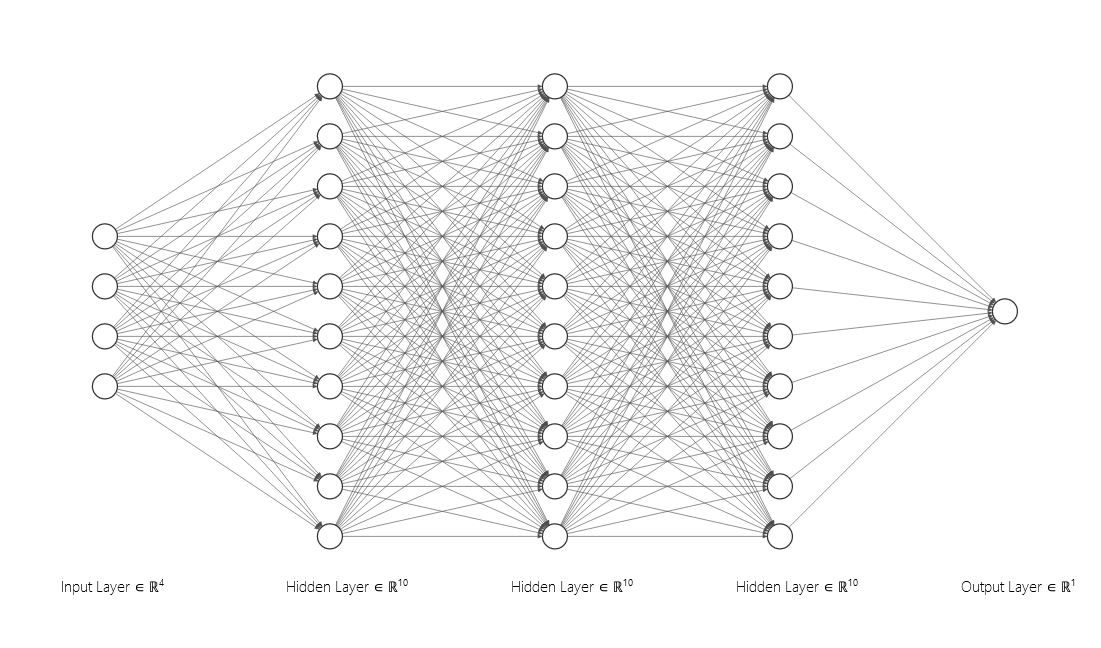
\includegraphics[scale=0.7]{Figures/nn_basic_fig.JPG}
    \rule{35em}{0.5pt}
  \caption[Vanilla Neural Network]{Basic Neural Network}
  \Source{https://alexlenail.me/NN-SVG/}
  \label{fig:basic_nn}
\end{figure}

DNNs consists of mainly three components:
\begin{itemize}[noitemsep,topsep=0pt]
    \item Input Layer
    \item \textit{n} number of Hidden Layers
    \item Output Layer
\end{itemize}

The input layer is the first layer in the network and is responsible for taking in the input. This input is then passed on to the next hidden layer, and so on until the last hidden layer. From the last hidden layer, the information is passed on to the output layer. At the output layer, the model output is used to calculate the loss. The loss is a measure of how far off the prediction of the network is as compared to the actual output. This loss is then backpropagated through the neural network thus updating the model weights.

% Welcome to this \LaTeX{} Thesis Template, a beautiful and easy to use template for writing a thesis using the \LaTeX{} typesetting system.

% If you are writing a thesis (or will be in the future) and its subject is technical or mathematical (though it doesn't have to be), then creating it in \LaTeX{} is highly recommended as a way to make sure you can just get down to the essential writing without having to worry over formatting or wasting time arguing with your word processor.

% \LaTeX{} is easily able to professionally typeset documents that run to hundreds or thousands of pages long. With simple mark-up commands, it automatically sets out the table of contents, margins, page headers and footers and keeps the formatting consistent and beautiful. One of its main strengths is the way it can easily typeset mathematics, even \emph{heavy} mathematics. Even if those equations are the most horribly twisted and most difficult mathematical problems that can only be solved on a super-computer, you can at least count on \LaTeX{} to make them look stunning.

%----------------------------------------------------------------------------------------


% Chapter 3

\chapter{Literature Review} % Main chapter title

\label{Chapter3} % For referencing the chapter elsewhere, use \ref{Chapter3} 

\lhead{Chapter 3. \emph{Literature Review}} % This is for the header on each page - perhaps a shortened title

%----------------------------------------------------------------------------------------
In the recent years, research in mathematical finance has started incorporating AI based methods in addition to existing traditional models. This chapter looks at previous work in pricing options using deep learning. 

In a paper titled “Machine Learning in Finance:The Case of Deep Learning for Option Pricing“\cite{Culkin2017MachineLI}, Culkin and Das experimented with a basic Neural Network model consisting of 4 hidden layers containing 100 neurons each. Even with such a basic model, they were able to achieve an RMSE of 0.0112 and a 4\% option pricing error for both In-sample and Out-of-sample options. In addition to the low error, they also reported an R2 value of 0.9982, which is very high. Their study showed promising results for neural networks in option pricing.

Herzog and Osamah's 2019 paper "Reverse Engineering of Option Pricing: An AI Application"\cite{Herzog2019ReverseEO} uses a genetic algorithm approach to model option prices in the German market. Their results show that their RE (Reverse Engineering) model outperformed the Black-Scholes model 2740/2791 times, or more than 98\% of the time. This paper is shows how Fuzzy logic and Artificial Intellignce based approaches are starting to outperform models like Black-Scholes and Heston by leveraging more data and improving software and hardware.


In "Pricing options and computing implied volatilities using neural networks"\cite{risks7010016}, the authors try something different by comparing the PDE models to Neural Network models. They use different methods like Black-Scholes model, Heston model and Brent method to generate a large number of option prices and then train Neural networks using different numbers of layers, neurons, etc. to reproduce the results of these methods. This provides a huge advantage in terms of speed and accuracy since Neural Networks are much more parallelizable as compared to PDE based solvers.

Das in his 2016 article\cite{10.1007/s00521-016-2303-y} proposes and investigates a hybrid model that combines parametric option pricing models (such as the Black–Scholes option pricing model) with non-parametric machine learning techniques (such as support vector regression and extreme learning machine-based regression models). The main advantages of this hybrid approach are that it can focus on nonlinear approximation, learn the mechanism of the options market by understanding the key features embedded in the parametric models, and reduce forecasting error by using non-parametric models. Additionally, this approach can reduce the influence of seasonality in data and reduce computational complexity by using a smaller group of data for predictions.


Goswami\cite{Goswami2020DatadrivenOP} in his recent work on pricing options of Indian market indices, explores the use of supervised machine-learning algorithms to price European-style call options. Three different approaches are proposed, each of which yields a range of fair prices rather than a single price point. The model performance is tested on two stock market indices: NIFTY50 and BANKNIFTY from the Indian equity market. In total, 17-22 features are generated from the market data, which are then used to train two models - an Artificial Neural Network and the XGBoost algorithm respectively.
% Chapter 4

\chapter{Dataset} % Main chapter title

\label{Chapter4} % For referencing the chapter elsewhere, use \ref{Chapter3} 

\lhead{Chapter 4. \emph{Dataset}} % This is for the header on each page - perhaps a shortened title

%----------------------------------------------------------------------------------------
\section{NIFTY 50}

The NIFTY 50 is the main index on the National Stock Exchange of India Ltd. (NSE). It tracks the performance of a selection of the biggest and most liquid Indian securities, including 50 of the approximately 1600 companies traded on NSE. This index covers around 65\% of the market's float-adjusted capitalization and is a good representation of the overall Indian stock market.
NIFTY 50 index covers a broad range of sectors in the Indian economy and provides investment managers with exposure to the Indian market in a single, efficient portfolio. It has been trading since 1996 and is ideal for benchmarking index funds and index-based derivatives. Using this index as the underlying asset, NIFTY index options were created.

\section{Data Collection}
\subsection{NIFTY Option Data}

\begin{figure}[htbp]
  \centering
    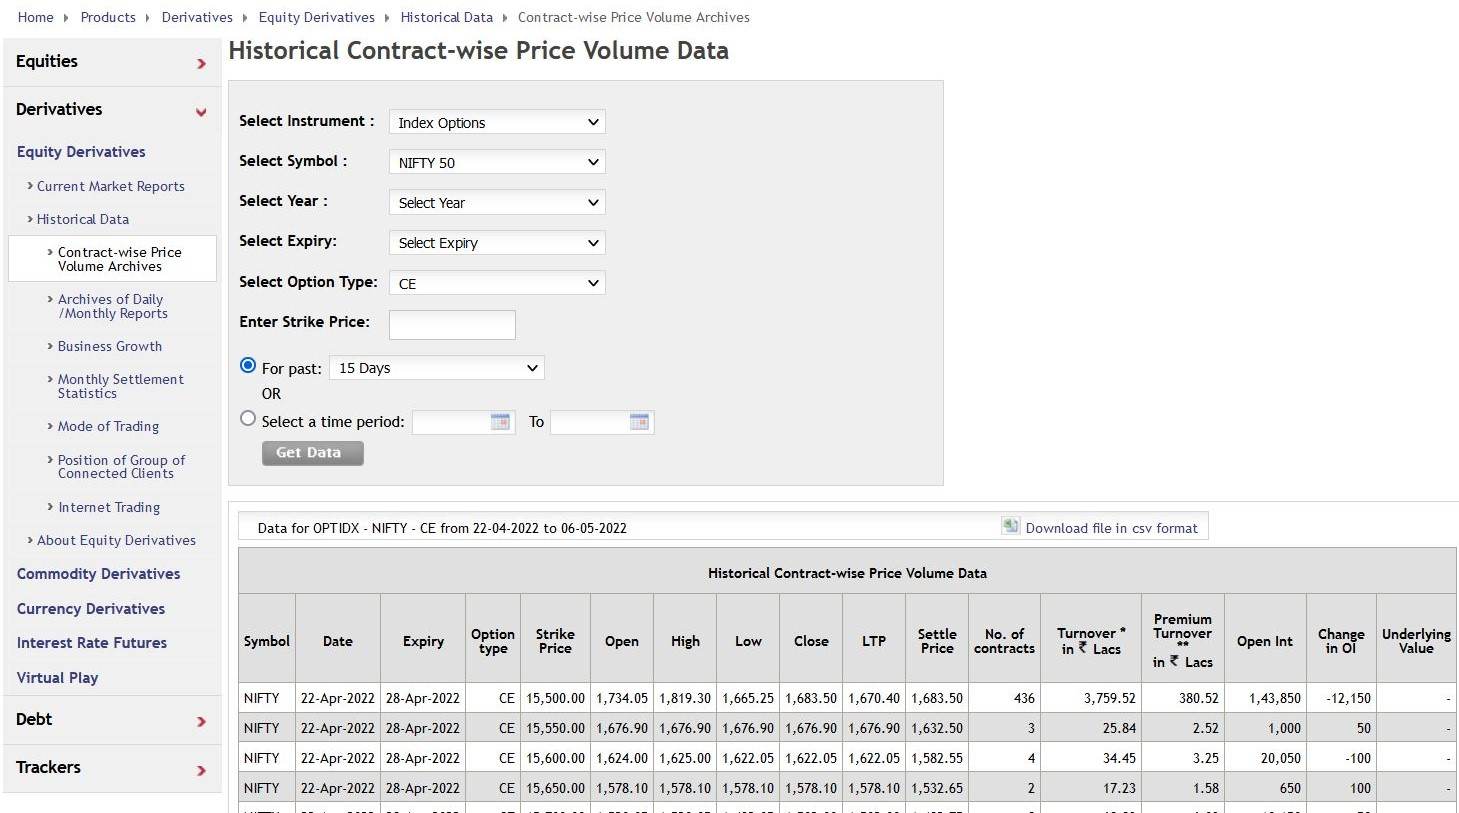
\includegraphics[scale=0.35]{Figures/data_collec_nifty_option.JPG}
    \rule{35em}{0.5pt}
  \caption[NIFTY Index Options]{NIFTY Index Options - Historical Data}
  \label{fig:data_collec_nifty_option}
\end{figure}

Data for NIFTY index options is available on the \href{https://www1.nseindia.com/products/content/derivatives/equities/historical_fo.htm}{NSE} website. The data used in this work contains information related to the NIFTY index put and call options between 2017 and 2022. Since the NSE website does not support scraping or downloading more than 90 consecutive days worth of data, data has been manually downloaded and combined for the target duration.
\\
\\

Figure ~\ref{fig:data_collec_nifty_option} shows a snapshot of the NSE website from which the option data has been downloaded.

\subsection{NIFTY Index Value}

Value of the underlying asset is an important piece of information for any derivative. While the option data contains a lot of information, the value of the underlying asset i.e. NIFTY index value, is not available for all the rows. To address this, the NIFTY index data for the same duration has also been downloaded from the \href{https://www1.nseindia.com/products/content/equities/indices/historical_index_data.htm}{NSE} webiste.

\begin{figure}[htbp]
  \centering
    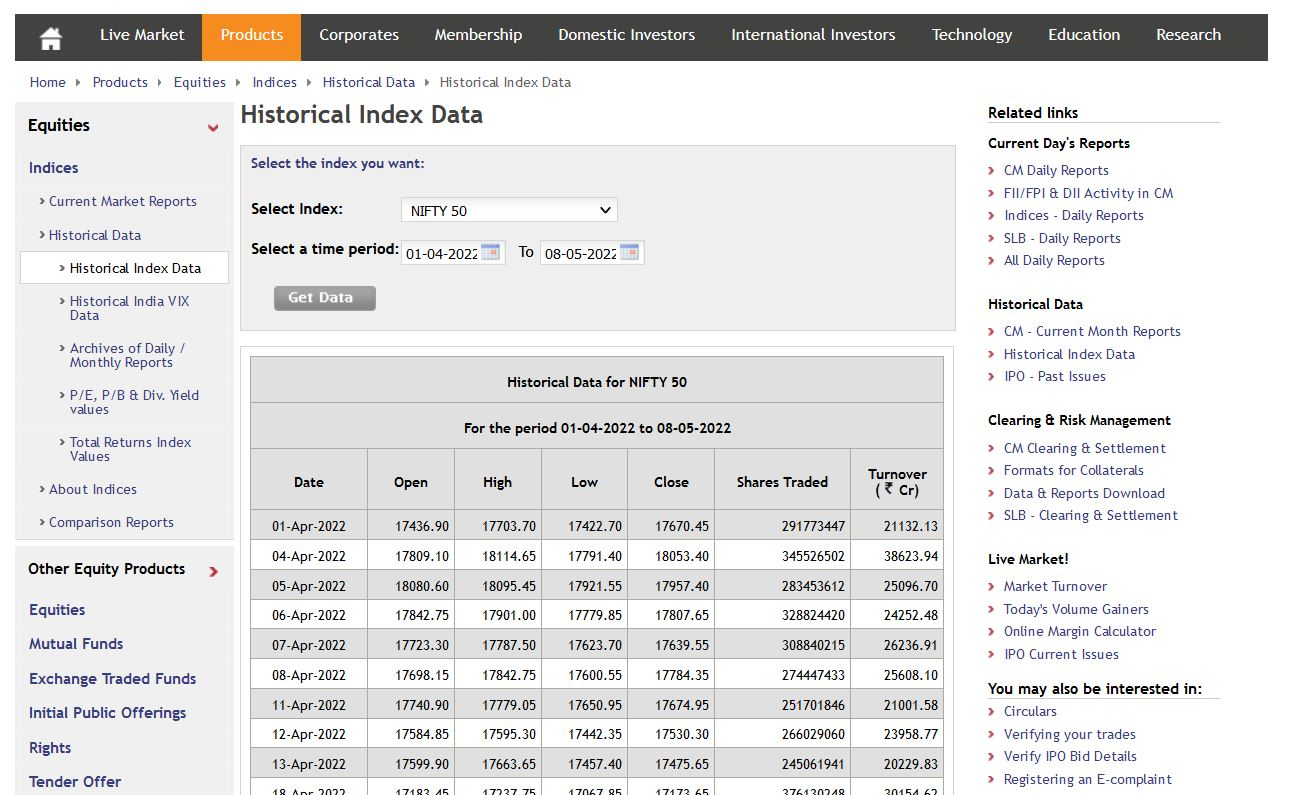
\includegraphics[scale=0.35]{Figures/data_collec_nifty_index.JPG}
    \rule{35em}{0.5pt}
  \caption[NIFTY Index Value]{NIFTY Index Value - Historical Data}
  \label{fig:data_collec_nifty_index}
\end{figure}

Figure ~\ref{fig:data_collec_nifty_index} shows a snapshot of the NSE website from which the index data has been downloaded.

\subsection{Risk Free Rate}

For risk free rate, yield of the 10 year government bond is used.   

\begin{figure}[htbp]
  \centering
    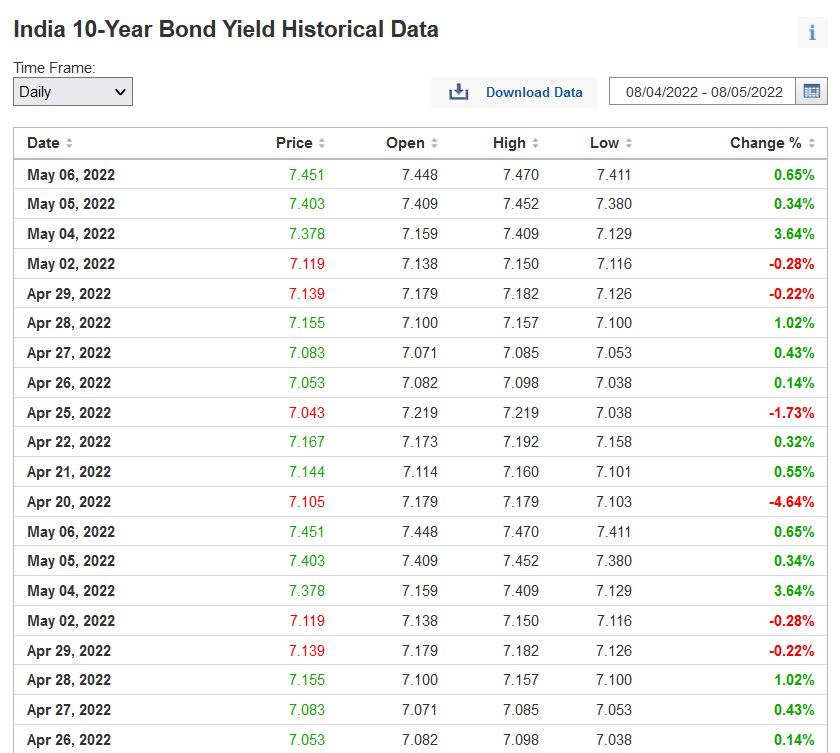
\includegraphics[scale=0.35]{Figures/data_collec_risk_rate.JPG}
    \rule{35em}{0.5pt}
  \caption[Risk Free Rate]{Risk Free Rate - Historical Data}
  \label{fig:data_collec_risk_rate}
\end{figure}

Figure ~\ref{fig:data_collec_risk_rate} shows past values of risk free rate in the context of Indian markets.

\section{Data Preparation}

Since all the data is currently in different CSV files, it needs be cleaned, prepared and merged to get the final data which will be used in the Neural Network and Black-Scholes model. Firstly, the duration needs to be calculated. To achieve this, we subtract the current date from the option expiry data and to normalize this duration, we divide it by 252, which is the number of trading days in a year. 

\begin{figure}[htbp]
  \centering
    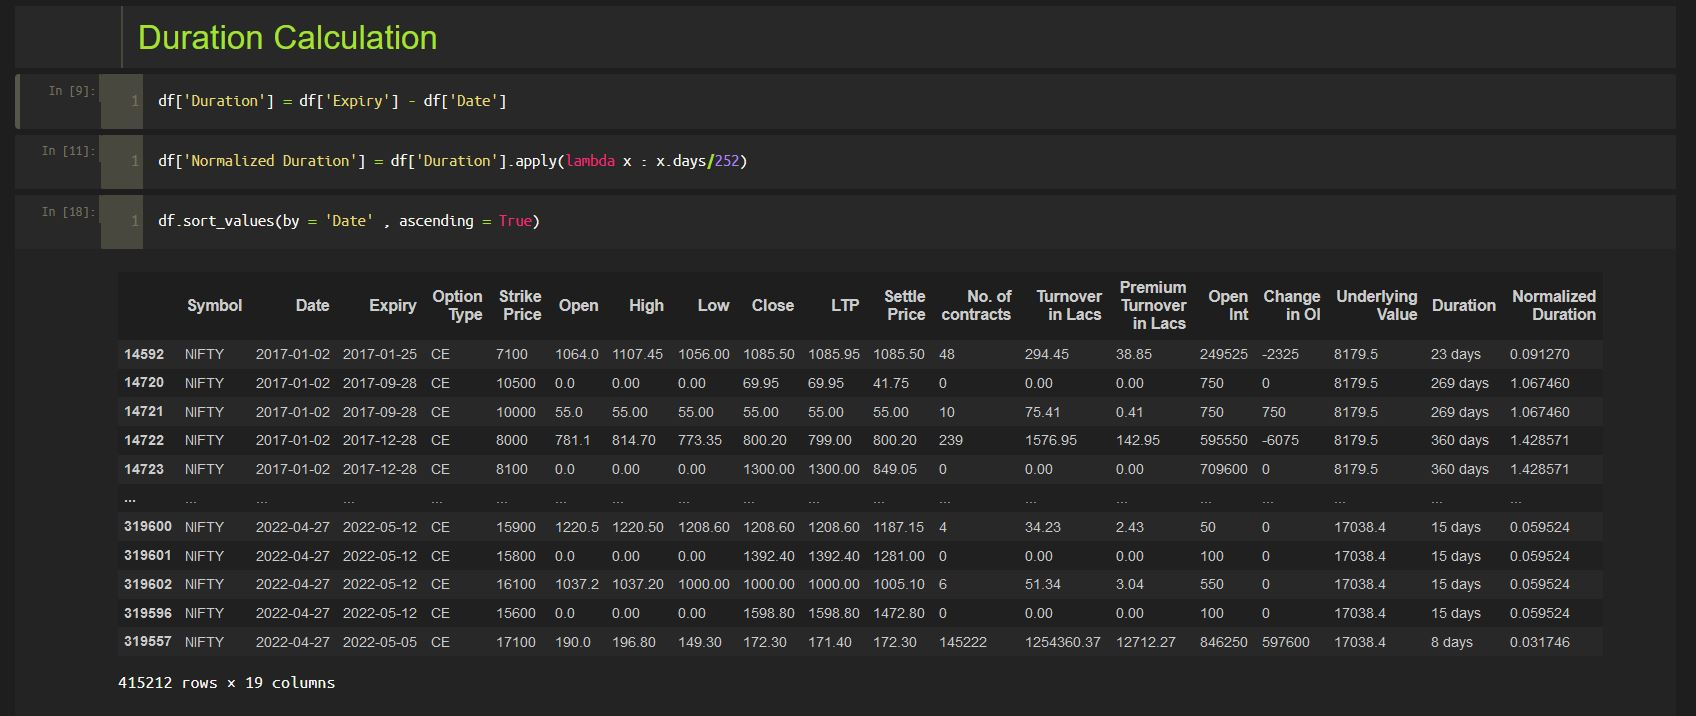
\includegraphics[scale=0.42]{Figures/data_prep_duration.JPG}
    \rule{35em}{0.5pt}
  \caption[Duration Calculation]{Duration}
  \label{fig:data_prep_duration}
\end{figure}

Apart from duration, volatility of the underlying asset is also an important feature for predicting the option premium. A 6 day window is chosen to calculate returns on the NIFTY index throughout each year. The standard deviation of this return for that particular year multiplied by $\sqrt{252}$ is used as historical volatility (sigma) in the models.

Figure ~\ref{fig:data_prep_volat} shows the code for calculating volatility. 

\begin{figure}[htbp]
  \centering
    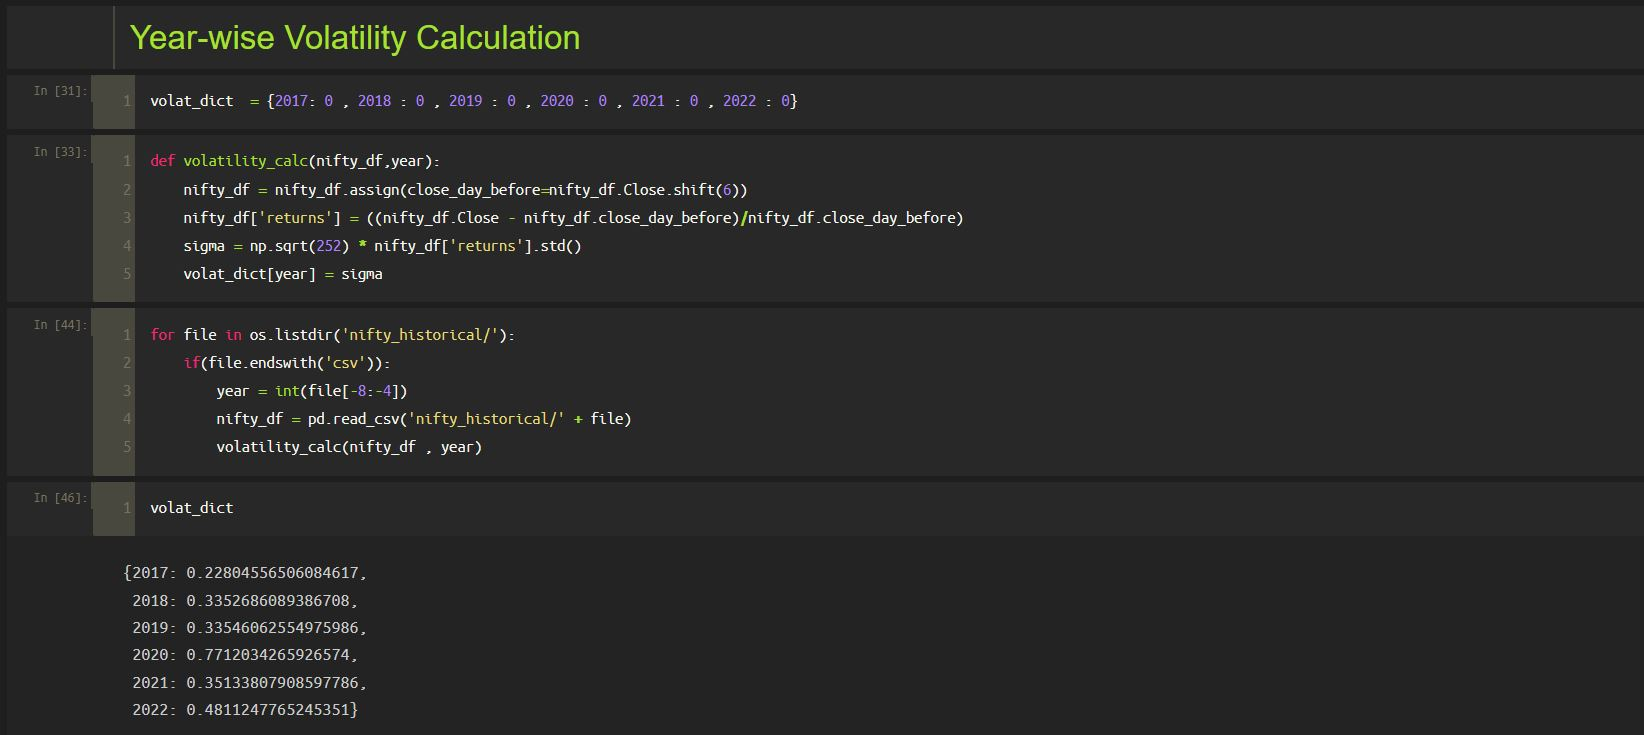
\includegraphics[scale=0.45]{Figures/data_prep_volat.JPG}
    \rule{35em}{0.5pt}
  \caption[Volatility Calculation]{Volatility}
  \label{fig:data_prep_volat}
\end{figure}

Finally, all this data is merged into one single dataframe which can be directly fed into the models.

\begin{figure}[htbp]
  \centering
    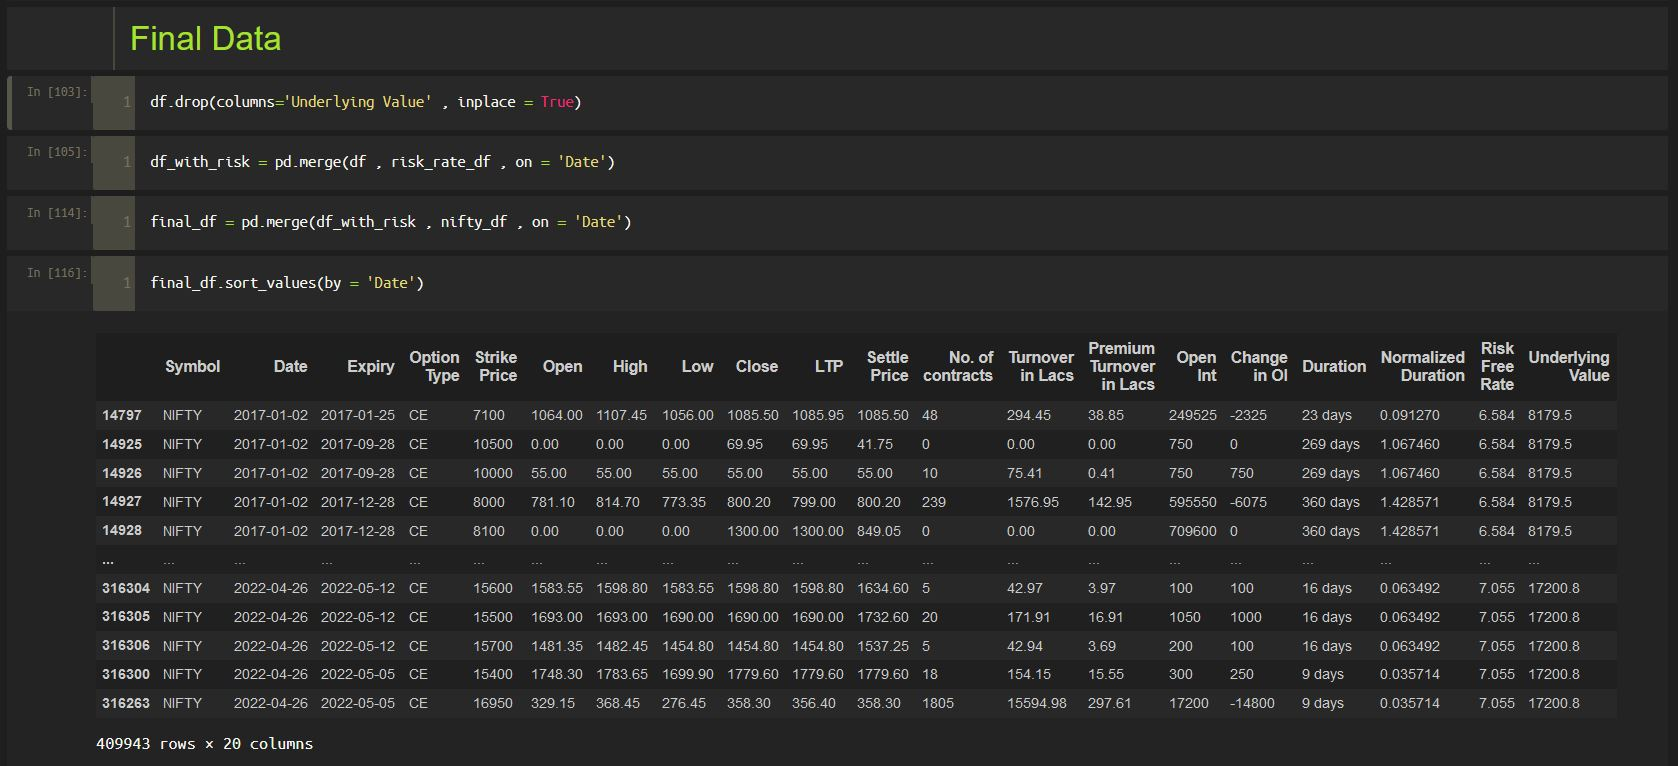
\includegraphics[scale=0.44]{Figures/data_prep_final.JPG}
    \rule{35em}{0.5pt}
  \caption[Final Data]{Final Data}
  \label{fig:data_prep_final}
\end{figure}

Figure ~\ref{fig:data_prep_final} shows the code for merging all the previous dataframes into the final dataframe. 


% Chapter Template

\chapter{Result and Discussion} % Main chapter title

\label{Chapter5} % Change X to a consecutive number; for referencing this chapter elsewhere, use \ref{ChapterX}

\lhead{Chapter 5. \emph{Result and Discussion}} % Change X to a consecutive number; this is for the header on each page - perhaps a shortened title

%----------------------------------------------------------------------------------------
%	SECTION 1
%----------------------------------------------------------------------------------------

\section{Results}

The results from all the models that have been introduced previously are discussed in this section.

\subsection{Full Data}

All the baseline models were run on the full dataset (600k rows). They do not use anything other than the mail text as input. 
\begin{table}[!h]
\captionsetup{textfont = large}
\caption{Baseline Results - Full Data}
\label{tab:baseline_full_results}
\begin{center}
\resizebox{0.75\textwidth}{!}{
\begin{tabular}{|l|r|r|r|r|}
\hline
\textbf{Model}   & \multicolumn{1}{l|}{\textbf{Majority F1}} & \multicolumn{1}{l|}{\textbf{Minority F1}} & \multicolumn{1}{l|}{\textbf{Macro F1}} & \multicolumn{1}{l|}{\textbf{Accuracy}} \\ \hline
\rowcolor[HTML]{C0C0C0} 
SVM + tfidf      & 0.819                                     & 0.19                                      & 0.505                                  & 0.705                                  \\ \hline
CNN              & 0.827                                     & 0.163                                     & 0.495                                  & 0.713                                  \\ \hline
\rowcolor[HTML]{C0C0C0} 
LSTM             & 0.827                                     & 0.178                                     & 0.503                                  & 0.714                                  \\ \hline
BiLSTM           & 0.827                                     & 0.183                                     & 0.505                                  & 0.715                                  \\ \hline
\rowcolor[HTML]{C0C0C0} 
LSTM + Attention & 0.828                                     & 0.179                                     & 0.503                                  & 0.715                                  \\ \hline
BERT             & 0.827                                     & 0.215                                     & 0.521                                  & 0.716                                  \\ \hline
\rowcolor[HTML]{C0C0C0} 
RoBERTa          & 0.826                                     & \textbf{0.232}                            & \textbf{0.529}                         & \textbf{0.717}                         \\ \hline
\end{tabular}
}
\end{center}
\end{table}

RoBERTa outperforms all the other baseline models on all metrics except Majority F1. Since the other features are not available for the full data, the MultiModal models have not been included in Table~\ref{tab:baseline_full_results}.

\subsection{MultiModal Data}

Using 18K rows from the full data, this subset is created which contains 135 other non-text features apart from the email body. Results from the models that were run on this data are presented in Table~\ref{tab:18k_data_results}

\begin{table}[!h]
\captionsetup{textfont = large}
\caption{Model Results - 18K Data}
\label{tab:18k_data_results}
\begin{center}
\resizebox{0.85\textwidth}{!}{
\begin{tabular}{|l|r|r|r|}
\hline
\textbf{Model}                           & \multicolumn{1}{l|}{\textbf{Minority F1}} & \multicolumn{1}{l|}{\textbf{Macro F1}} & \multicolumn{1}{l|}{\textbf{Accuracy}} \\ \hline
SVM + tfidf                              & 0.263                                     & 0.528                                  & 0.677                                  \\ \hline
CNN                                      & 0.240                                     & 0.524                                  & 0.693                                  \\ \hline
LSTM                                     & 0.133                                     & 0.481                                  & 0.713                                  \\ \hline
BiLSTM                                   & 0.186                                     & 0.507                                  & 0.716                                  \\ \hline
LSTM + Attention                         & 0.034                                     & 0.433                                  & 0.713                                  \\ \hline
BERT                                     & 0.272                                     & 0.546                                  & 0.712                                  \\ \hline
RoBERTa                                  & 0.272                                     & 0.548                                  & 0.716                                  \\ \hline
BERT + LIWC + Politeness + Topic         & 0.085                                     & 0.461                                  & 0.724                                  \\ \hline
BERT + Interpersonal Context             & 0.257                                     & 0.555                                  & 0.754                                  \\ \hline
BERT + Interpersonal Context + Influence & \textbf{0.264}                            & \textbf{0.559}                         & \textbf{0.757}                         \\ \hline
\end{tabular}
}
\end{center}
\end{table}

It is evident from the results that these non-text features do have the power to improve the model by providing more context about the mail, the sender and the receiver. While the model with LIWC, Politeness and Topic features are only $\sim$1\% more accurate than RoBERTa, the other MultiModal models are upto $\sim$4\% more accurate.


\section{Discussion}

As seen in Table~\ref{tab:baseline_full_results} and \ref{tab:18k_data_results}, the MultiModal models perform better than all the baseline models, beating the most capable model (RoBERTa) by more than $\sim$4\% in terms of accuracy. Comparing the different MultiModal models, we see that adding Influence features to BERT with Interpersonal Context features results in a small improvement. 

Another observation from the above results is that while features like LIWC and Politeness, which capture different stylistic properties about the text, do increase the accuracy of the model but not nearly as much as features like Interpersonal Context, which provide information about the linguistic style of the sender and receiver.  

Further work needs to be done to figure out the kind of features which lead to this increase in the model performance.
% Chapter Template

\chapter{Conclusion} % Main chapter title

\label{Chapter6} % Change X to a consecutive number; for referencing this chapter elsewhere, use \ref{ChapterX}

\lhead{Chapter 6. \emph{Conclusion}} % Change X to a consecutive number; this is for the header on each page - perhaps a shortened title

%----------------------------------------------------------------------------------------
%	SECTION 1
%----------------------------------------------------------------------------------------

\section{Recommendation for Future Research}

In the past few years, Graph Neural Networks (GNNs) have gained a lot of popularity. Traditional Deep Learning based models like CNNs and RNNs work on data like Images and Text, which can be regarded as Euclidean data. GNNs extend the power of these models to graph data which is non-Euclidean in nature. Molecular structure of proteins and people in a social graph can be considered as examples of non-Euclidean data. GNNs have also achieved great success in tasks on similar datasets in the recent years\cite{Wu2020GraphCN,fout2017protein}. This has made GNNs an active research topic in Artificial Intelligence today leading to new and improved graph based models like Graph Convolutional Network (GCN)\cite{kipf2017semi} and Graph Attention Network\cite{velickovic2018graph}.

% Since the Luxury-Standard data can also be modelled as a Social Graph, there is reason to believe Graph Neural Networks may perform well on this data.

The Luxury-Standard dataset contains information about both - the emails sent by the employees and the mail content. This means that the current data can be modelled as a social network graph after which a GNN can be applied to it. The advantage of GNNs is that they are able to leverage information from the neighbour nodes in the social graph similar to how a CNN exploits the spatial data in an image by looking at the adjacent pixels when sliding a window over the input. 

The data can be represented as a graph by converting each employee and mail as a node in a heterogeneous graph. For each $e_t : s \rightarrow r$, an edge is constructed between $s$-$e_t$ and $r$-$e_t$. A design choice over here can give rise to two different kind of graphs - one containing an edge between $s$-$r$ and another one without any $s$-$r$ edge. 

\clearpage

\begin{figure}[!tbp]
  \centering
\subfloat[Without Sender-Receiver Edge]{    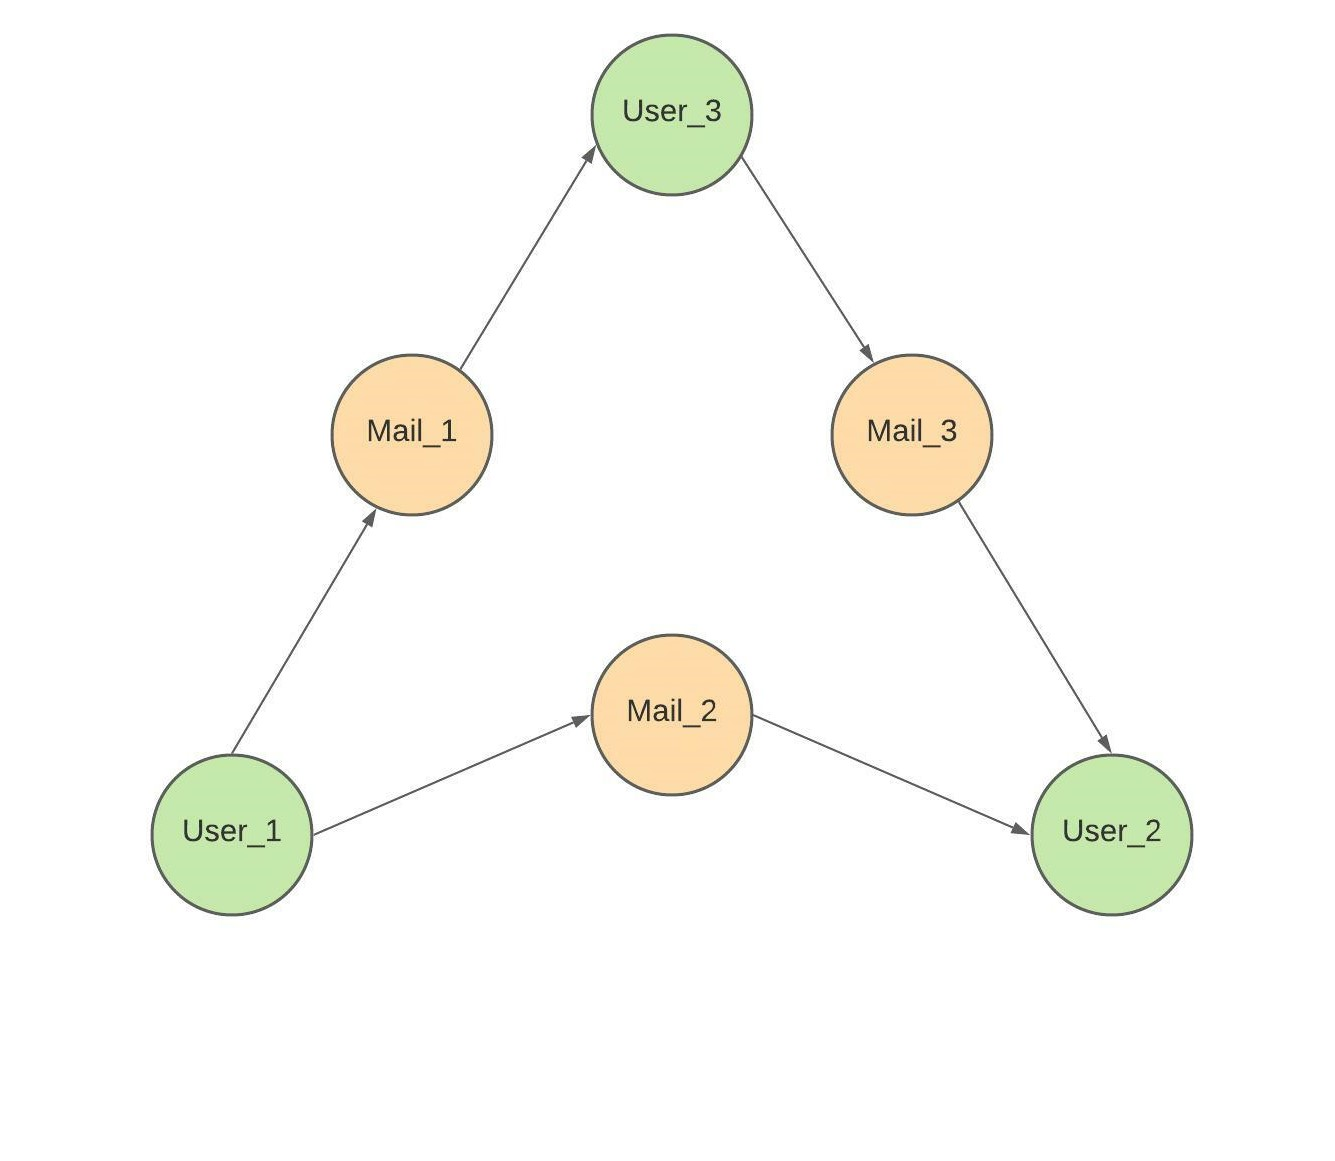
\includegraphics[width=0.48\textwidth]{Figures/graph_type_1.jpeg}} 
\subfloat[With Sender-Receiver Edge]{    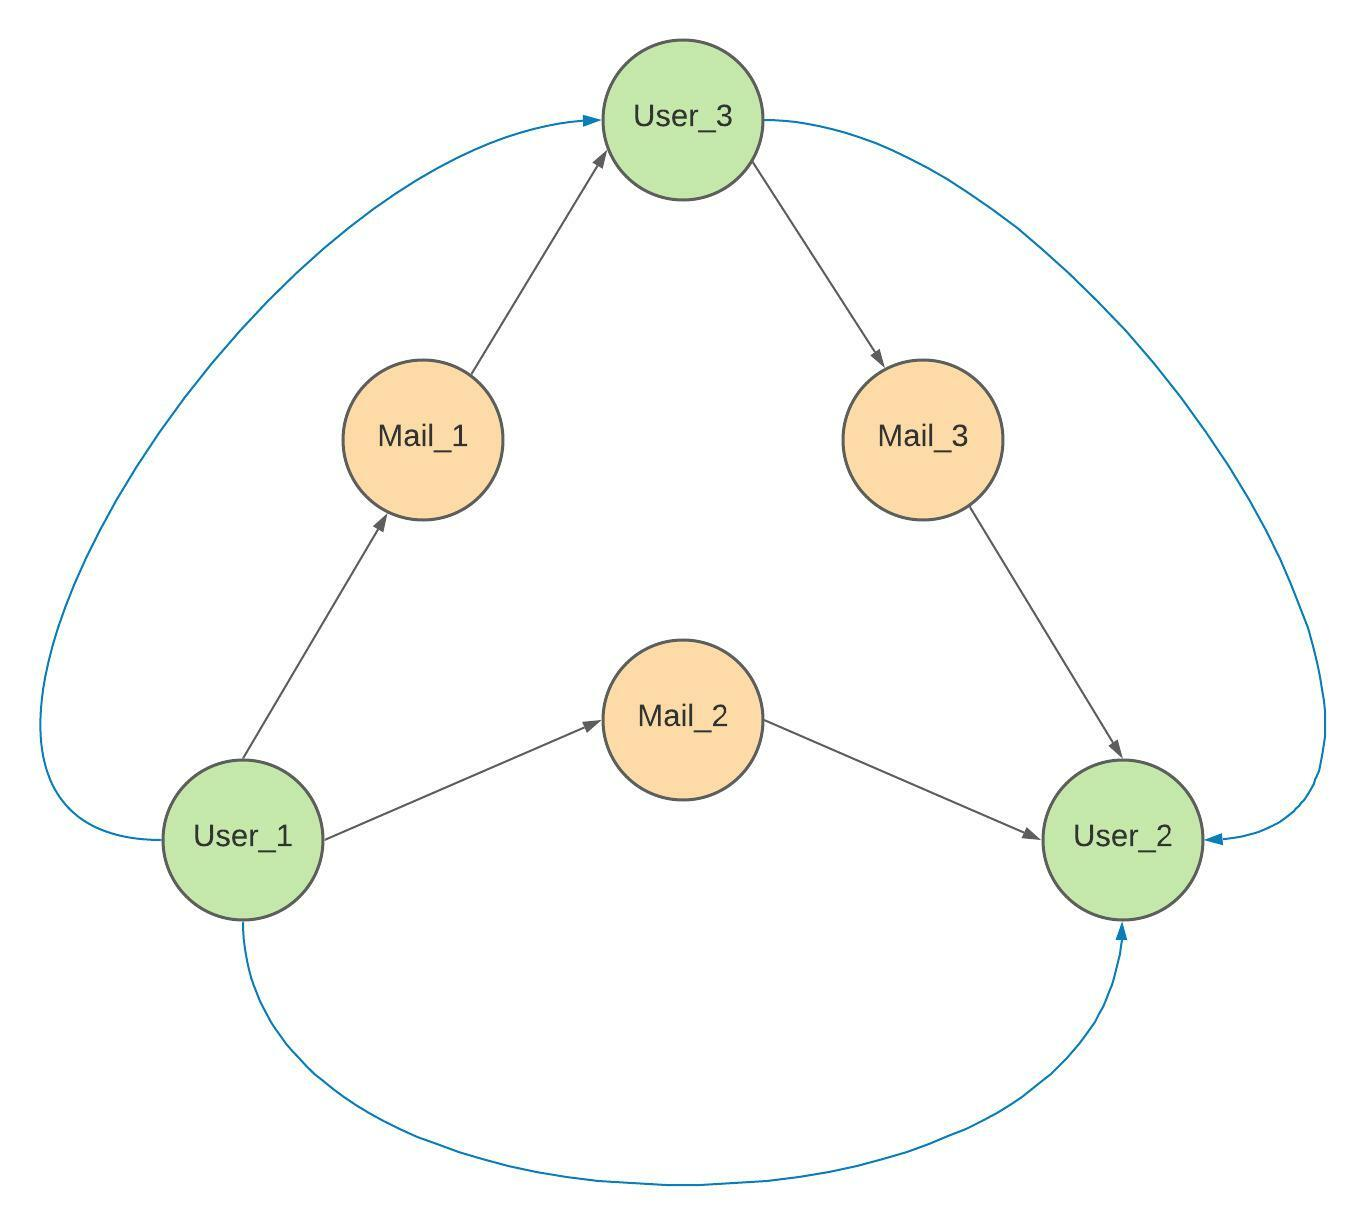
\includegraphics[width=0.48\textwidth]{Figures/graph_type_2.jpeg}}
    \caption{Data as Heterogeneous Graph}
  \label{fig:data_as_graph}
\end{figure}


Figure~\ref{fig:data_as_graph} shows an example of how the graph would look if created using either of the above mentioned methods. Once the data is in a compatible format, graph based machine learning libraries like PyTorch-Geometric\cite{Fey/Lenssen/2019} and StellarGraph\cite{StellarGraph} can be used to apply State-of-the-Art graph based methods on it.

\section{Conclusion}

Predicting the probability of getting a reply to a corporate mail would help the employees plan better. It can also help them write emails which are more likely to get a reply. The email body contains a lot of information that could help predict the chances of getting a reply back. But looking beyond this, we can see that there are many more factors involved like preferences of the sender and receiver, their workplace relations with each other, style of the message, and so on.

Incorporating these various features along with the email body cannot be done in a simple Transformer model like BERT which works solely on textual input. The proposed MultiModal architecture addresses this issue by using BERT to generate embeddings for the email body which is then concatenated with other numerical and categorical features to form the final email representation. These changes improve the accuracy by more than $\sim$4\% as compared to purely text based methods like BERT and RoBERTa.
%\input{Chapters/Chapter7}

%-------------------------------------------------------------------------------
%	THESIS CONTENT - APPENDICES
%-------------------------------------------------------------------------------

\addtocontents{toc}{\vspace{2em}} % Add a gap in the Contents, for aesthetics

\appendix % Cue to tell LaTeX that the following 'chapters' are Appendices

% Include the appendices of the thesis as separate files from the Appendices
% folder
% Uncomment the lines as you write the Appendices

% Appendix A

\chapter{Code} % Main appendix title

\label{appendix_code} % For referencing this appendix elsewhere, use \ref{AppendixA}

\lhead{Appendix A. \emph{Code and Model Architectures}} % This is for the header on each page - perhaps a shortened title

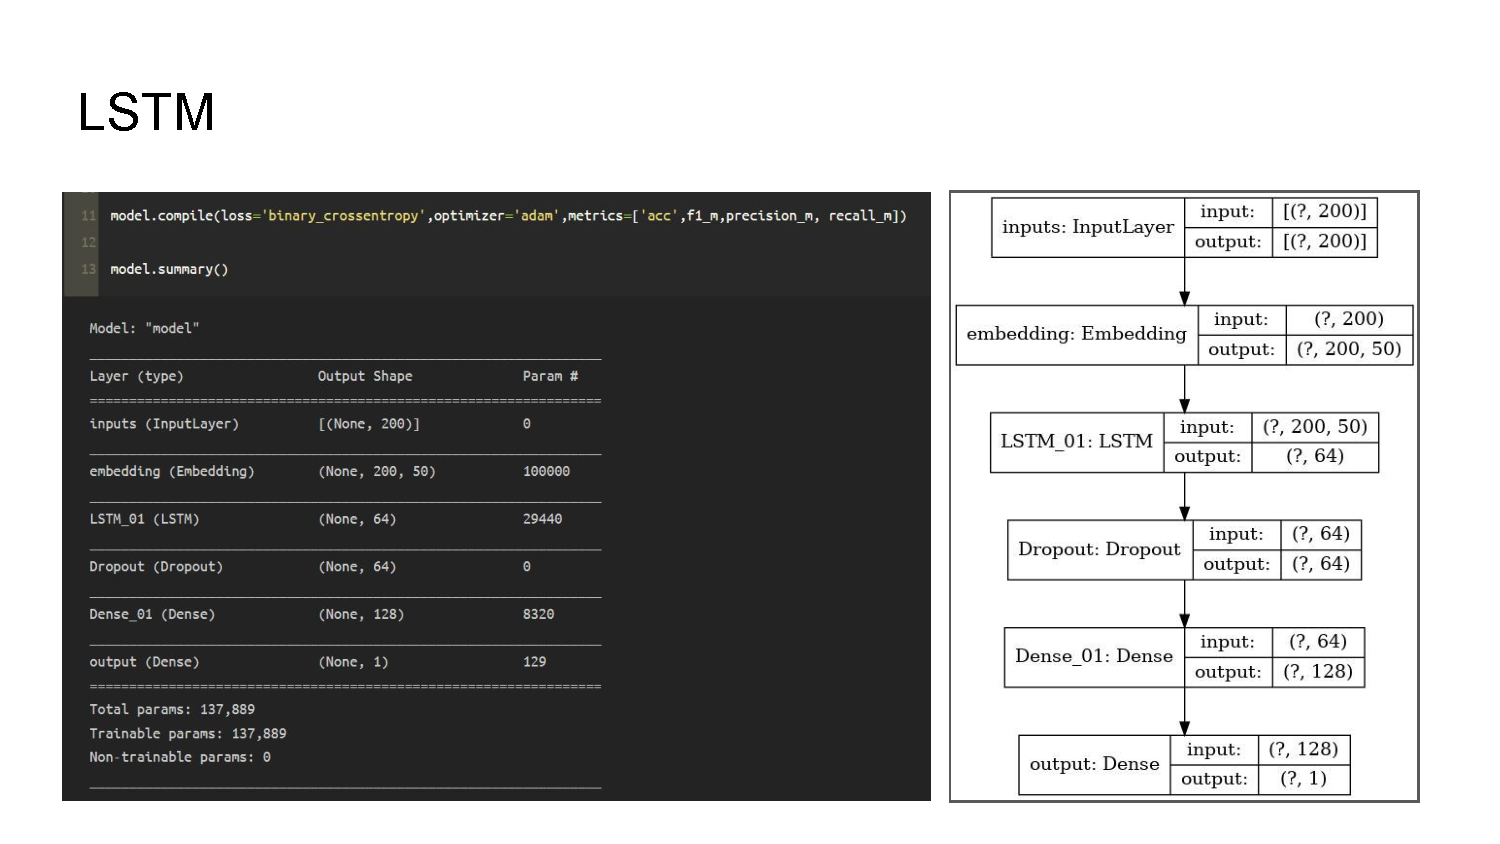
\includegraphics[page=1,width=1.1\textwidth,left]{Appendices/code_appendix.pdf}
\clearpage
\includegraphics[page=2,width=1.1\textwidth,left]{Appendices/code_appendix.pdf}
\newline
\newline
\includegraphics[page=3,width=1.1\textwidth,left]{Appendices/code_appendix.pdf}
\newpage
\includegraphics[page=4,width=1.1\textwidth,left]{Appendices/code_appendix.pdf}
\newline
\newline
\includegraphics[page=5,width=1.1\textwidth,left]{Appendices/code_appendix.pdf}
% Appendix Template

\chapter{Converting dataset from CSV to Graph} % Main appendix title

\label{AppendixB} % Change X to a consecutive letter; for referencing this appendix elsewhere, use \ref{AppendixX}

\lhead{Appendix B. \emph{Converting dataset from CSV to Graph}}
Currently, the dataset is in a CSV format which needs to be converted into a Graph format for which we can then feed into the GNN model.
To keep things simple for the baseline model, we model all the employees and EACH mail as a node in a heterogeneous graph containing two different node types. After this we create an edge between the following pairs:

\begin{itemize}[noitemsep,topsep=0pt]
    \item (sender, message)
    \item (receiver, message)
    \item (sender,receiver)
\end{itemize}

Mail node contains an attribute called reply which contains 0 or 1 based on whether this particular message received a reply or not.
The final graph created is an undirected heterogeneous multi-graph since the nodes are connected to multiple nodes.

\begin{center}
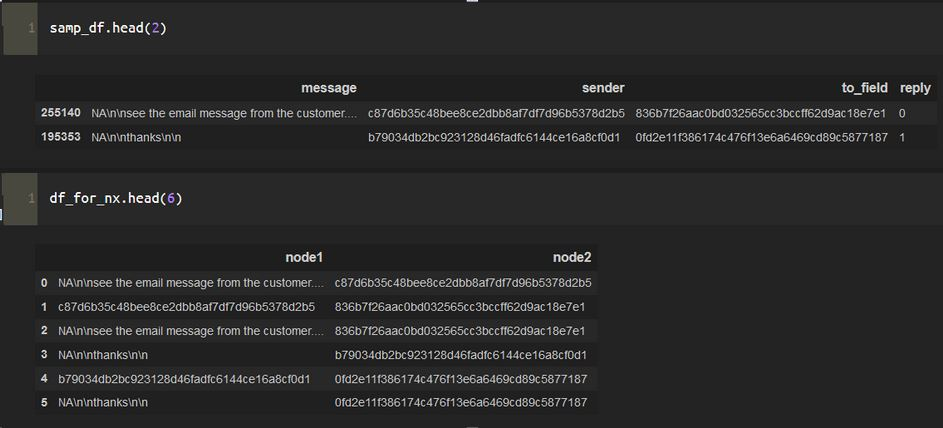
\includegraphics[scale=0.75]{Appendices/image1_graph.JPG}
\end{center}

To create the graph from CSV, the node pairs mentioned earlier need to be created. The code above shows the original dataframe and the new dataframe used to create the graph. They both contain the same data, just in different format
\begin{center}
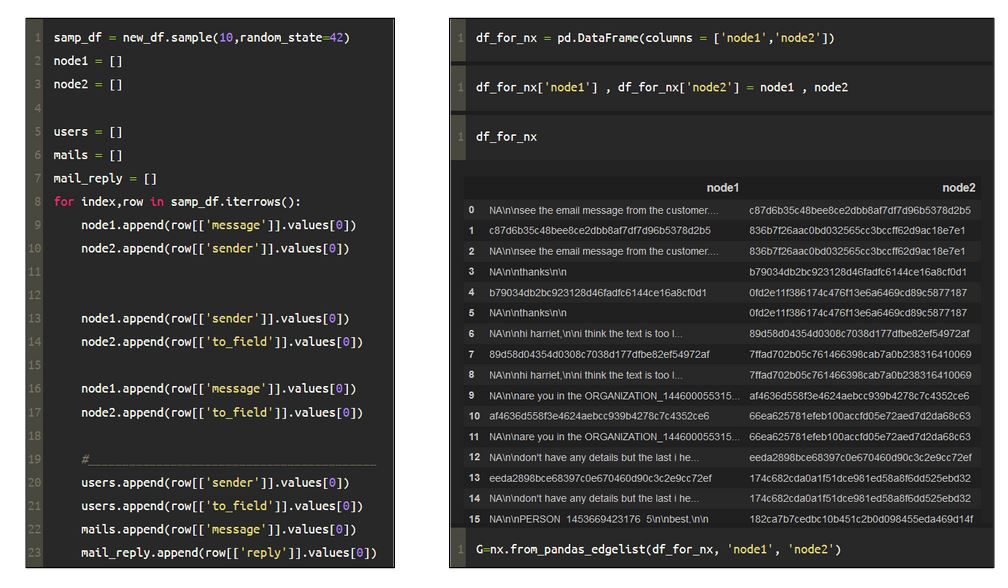
\includegraphics[scale=0.75]{Appendices/image2_graph.JPG}
\end{center}

Using this code, a networkx graph is created which can be used with a Graph Machine Learning Library.

\begin{center}
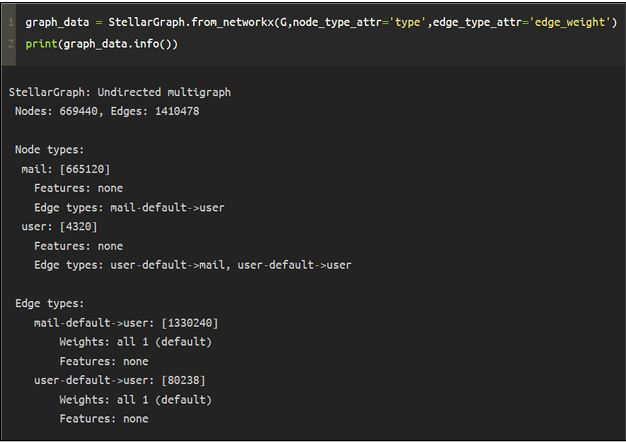
\includegraphics[scale=0.75]{Appendices/image3_graph.JPG}
\end{center}



%\input{Appendices/AppendixC}

\addtocontents{toc}{\vspace{2em}} % Add a gap in the Contents, for aesthetics

\backmatter

%-------------------------------------------------------------------------------
%	BIBLIOGRAPHY
%-------------------------------------------------------------------------------

\label{Bibliography}

\lhead{\emph{Bibliography}} % Change the page header to say "Bibliography"

\printbibliography

\end{document}
